\begin{figure}[!htb]
	\centering

	\begin{tikzpicture}

		\node (Delaunay) at (-3,0) {
			\begin{tikzpicture}[scale=0.15]
				\coordinate (1) at (-5,-8);
				\coordinate (2) at (10,2);
				\coordinate (3) at (10,10);
				\coordinate (4) at (-7,1);
				\coordinate (5) at (-1,8);
				\coordinate (6) at (-4,-9);
				\coordinate (7) at (5,-3);
				\coordinate (8) at (6,4);
				\coordinate (9) at (3,-5);
				\coordinate (10) at (0,1);
				\coordinate (O) at (-3.5,-2.94);

				\draw[rounded corners=1pt] (4) -- (5) -- (10) -- cycle;
				\draw[rounded corners=1pt] (1) -- (6) -- (9) -- cycle;
				\draw[rounded corners=1pt] (5) -- (8) -- (10) -- cycle;
				\draw[rounded corners=1pt] (7) -- (8) -- (10) -- cycle;
				\draw[rounded corners=1pt] (7) -- (9) -- (10) -- cycle;
				\draw[rounded corners=1pt] (2) -- (7) -- (8) -- cycle;
				\draw[rounded corners=1pt] (3) -- (5) -- (8) -- cycle;
				\draw[rounded corners=1pt] (2) -- (3) -- (8) -- cycle;
				\draw[red, thick, rounded corners=1pt] (1) -- (4) -- (10) -- cycle;

				\draw[dashed, blue] (O) circle[radius=5.27];

				\foreach \i in {1, ..., 10}{
						\filldraw[black] (\i) circle (4pt);
					}
				\filldraw[red] (1) circle (4pt);
				\filldraw[red] (4) circle (4pt);
				\filldraw[red] (10) circle (4pt);
			\end{tikzpicture}
		};

		\node (DelaunayText) at (-3, -3) {Respected};

		\node (NoDelaunay) at (3,0) {
			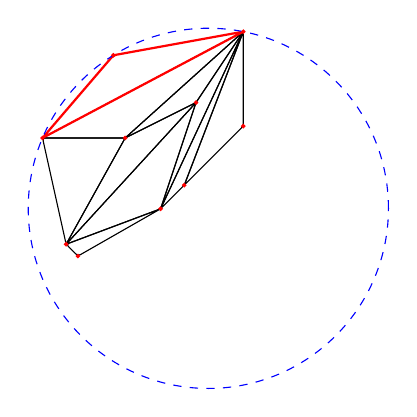
\begin{tikzpicture}[scale=0.15]
				\coordinate (1) at (-5,-8);
				\coordinate (2) at (10,2);
				\coordinate (3) at (10,10);
				\coordinate (4) at (-7,1);
				\coordinate (5) at (-1,8);
				\coordinate (6) at (-4,-9);
				\coordinate (7) at (5,-3);
				\coordinate (8) at (6,4);
				\coordinate (9) at (3,-5);
				\coordinate (10) at (0,1);
				\coordinate (O) at (7.04,-4.96);


				\draw[rounded corners=1pt] (4) -- (3) -- (10) -- cycle;
				\draw[rounded corners=1pt](3) -- (8) -- (10) -- cycle;
				\draw[rounded corners=1pt] (3) -- (2) -- (7) -- cycle;
				\draw[rounded corners=1pt] (3) -- (7) -- (9) -- cycle;
				\draw[rounded corners=1pt] (3) -- (8) -- (9) -- cycle;
				\draw[rounded corners=1pt] (8) -- (9) -- (1) -- cycle;
				\draw[rounded corners=1pt] (1) -- (4) -- (10) -- cycle;
				\draw[rounded corners=1pt] (1) -- (8) -- (10) -- cycle;
				\draw[rounded corners=1pt] (1) -- (6) -- (9) -- cycle;
				\draw[red, thick, rounded corners=1pt] (4) -- (3) -- (5) -- cycle;

				\draw[dashed, blue] (O) circle[radius=15.25];

				\foreach \i in {1, ..., 10}{
						\filldraw[red] (\i) circle (4pt);

					}
			\end{tikzpicture}
		};

		\node (NoDelaunayText) at (3, -3) {Not respected};

	\end{tikzpicture}

	\caption{Example for Delaunay condition}\label{fig:delaunayCondition}
\end{figure}
